% !TEX root = cha-application.tex
\documentclass[../../main.tex]{subfiles}

\begin{document}

\section{Minimum Distance Between Classes Comparison}
\label{sec:min_distance_comparison}

This experiment evaluates how the minimum class distance affects the execution time and success rate of WFC. The distance is measured as the Manhattan distance between class nodes on the grid. We used a subset of 9 classes from \texttt{JetUML} (shown in \figref{fig:minimum_distance_example}) and tested four minimum distances: 2, 3, 5, and 7 cells. For each distance, 24 solver instances were executed with a time limit of 24 hours.

\begin{figure}[ht]
    \centering
    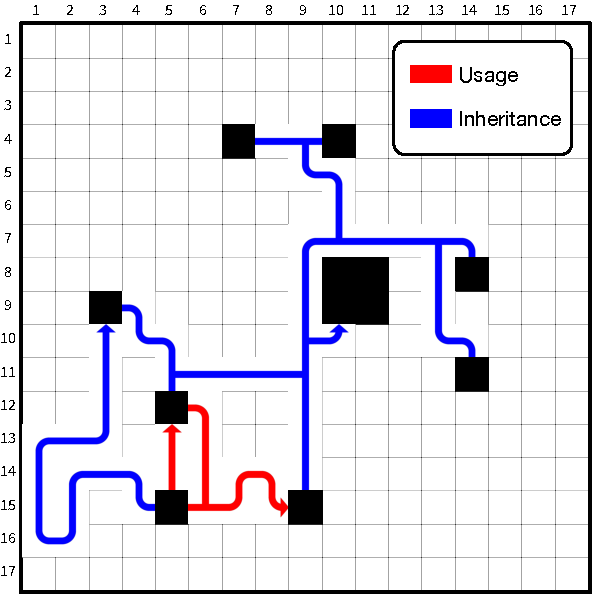
\includegraphics[width=0.46\linewidth]{figures/application/minimum_distance_example}
    \caption{Subset of 9 classes from the \texttt{org.jetuml.diagram} package.}
    \label{fig:minimum_distance_example}
\end{figure}

We expect that a larger minimum distance between classes requires a larger initial grid and longer paths between connected classes. This should increase the search space and make the generation more difficult.

The results are shown in \figref{fig:min_distance_results}. The boxplots in \figref{fig:min_distance_boxplot} clearly move towards higher execution times as the minimum distance increases. This shows that larger distances generally require more time to find a solution. Additionally, the cactus plot in \figref{fig:min_distance_cactus} displays the number of solved instances relative to execution time.

\begin{itemize}
    \item \textbf{Distance 2:} the average initial grid size is $17 \times 17$. 17 out of 24 instances were solved (70.8\%), with execution times between 38 seconds and approximately 44 minutes.

    \item \textbf{Distance 3:} the average initial grid size is $22 \times 22$. 19 out of 24 instances were solved (79.2\%), with execution times between 4 minutes and approximately 2 hours.

    \item \textbf{Distance 5:} the average initial grid size is $29.71 \times 29.71$. 6 out of 24 instances were solved (25.0\%), with execution times between 24 minutes and nearly 17 hours.

    \item \textbf{Distance 7:} the average initial grid size is $40.75 \times 40.75$. Only 1 out of 24 instances was solved (4.2\%), taking nearly 5 hours.
\end{itemize}

The results confirm this expectation. As the minimum distance increases, the initial grid becomes larger and the execution times generally increase. At the same time, the number of successful instances decreases.

\begin{figure}[ht]
    \centering
    \begin{subfigure}[b]{0.65\textwidth}
        \centering
        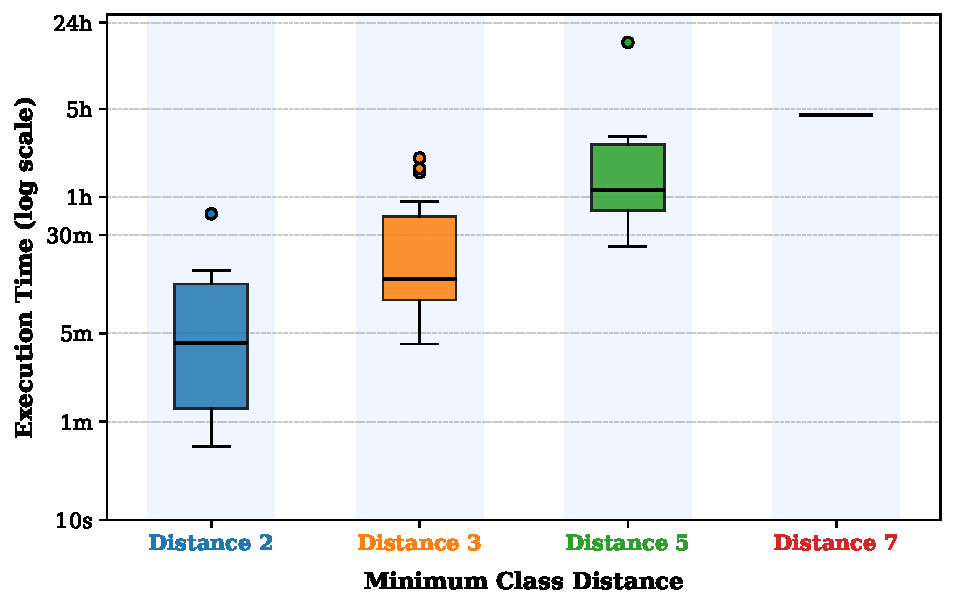
\includegraphics[width=\textwidth]{figures/application/min_distance_execution_times_boxplot}
        \caption{Execution times boxplot.}
        \label{fig:min_distance_boxplot}
    \end{subfigure}
    \hfill
    \begin{subfigure}[b]{0.65\textwidth}
        \centering
        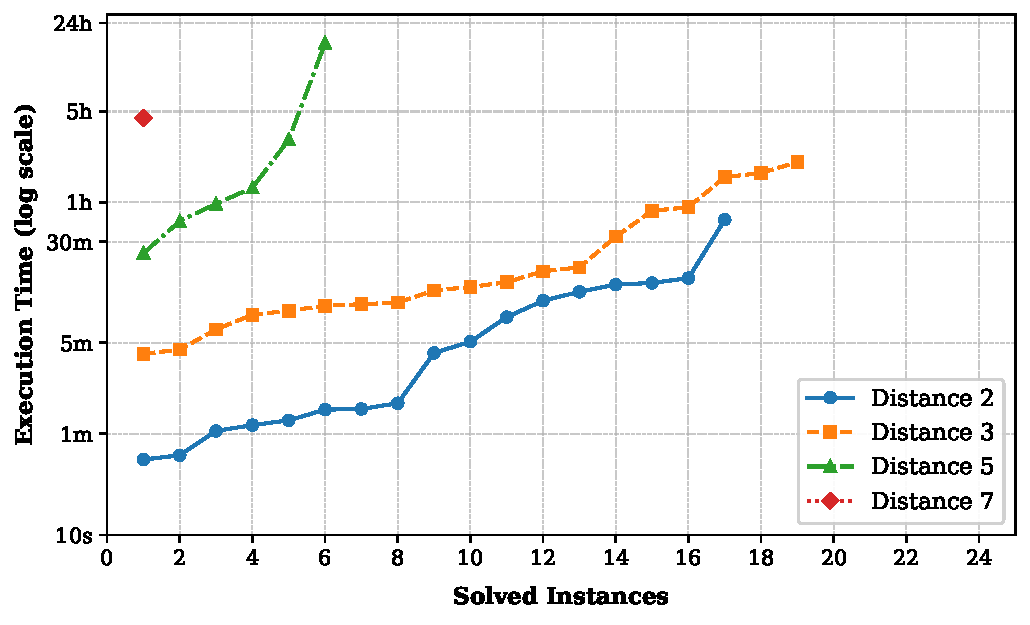
\includegraphics[width=\textwidth]{figures/application/min_distance_execution_times_cactus}
        \caption{Execution times cactus plot.}
        \label{fig:min_distance_cactus}
    \end{subfigure}
    \caption{Execution times for different minimum class distances.}
    \label{fig:min_distance_results}
\end{figure}

\end{document}